\lesson{Oct 11 2022}{Vectors}

\subsection{Formulation}
\label{sub:vector-formulation}

\begin{definition}[Vector]
    A mathematical object that has a:
    \begin{itemize}
        \item Magnitude
        \item Orientation
        \item Sense (sign)
    \end{itemize}
\end{definition}

We use arrows to represent vectors graphically, the choice of arrows is very similar to the choice of lengths to represent numbers.

\begin{figure}[H]
    \begin{center}
        \begin{tikzpicture}[scale=1, transform shape]
            \draw[thick, -{Latex}] (0,0) -- (2,2) node[above] {Sense};
            \draw[thick, -{Latex}] (0,0) -- (2,2) node[midway, above, rotate=45] {Magnitude};
            \fill (0,0) circle[radius=2pt];
            \draw[thick, dashed] (0,0) -- (-1, -1) node[below] {Direction};
        \end{tikzpicture}
    \end{center}
    \caption{A vector represented graphically using an arrow.}%
    \label{fig:vector}
\end{figure}

\begin{definition}[Vector equality]
    For $\vec{a}$ to be equal to $\vec{b}$
    \begin{itemize}
        \item $|\vec{a}| = |\vec{b}|$
        \item $\vec{a} \parallel \vec{b}$
        \item Sense of $\vec{a}$ is the same as that of $\vec{b}$
    \end{itemize}
\end{definition}

The choice of such an equality, although looks natural, is a made construct. This specific equality is useful for our calculations. However, it is as real as $\frac{1}{2}=\frac{3}{6}$, which, even though represents the notion of ratios, is not \textit{real} since, clearly, the process of cutting a pizza into 2 pieces is different from cutting it into 6 piece.

\begin{note}
    Equality is defined in terms of the original definition.
\end{note}

\subsection{Arithmetic}%
\label{sub:vector-arithmetic}

\subsubsection{Addition}%
\label{ssub:vector-addition}

\begin{definition}[Vector addition]
        Vector $\vec{a}+\vec{b}$ starts at the end of $\vec{A}$ and ends at the end of $\vec{B}$
\end{definition}

\begin{figure}[H]
    \begin{center}
        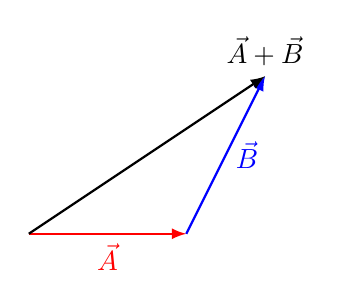
\begin{tikzpicture}[scale=1, transform shape]
            \draw[red,thick,-{latex}] (0,0) -- (2,0) node[midway, below]
                {$\vec{A}$};
            \draw[blue,thick,-{latex}] (2,0) -- (3,2) node[midway, right]
                {$\vec{B}$};
            \draw[thick,-{latex}] (0,0) -- (3,2) node[above]
                {$\vec{A}+\vec{B}$};
        \end{tikzpicture}
    \end{center}
    \caption{Sum of two vectors.}%
    \label{fig:vector-sum}
\end{figure}


This definition is based on the practicality of such a geometrical construct according to real life observations. Moreover, this enables commutative and associative.

\begin{figure}[htpb]
    \begin{center}
        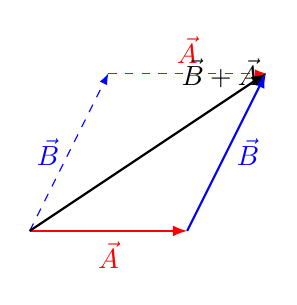
\begin{tikzpicture}[scale=1, transform shape]
            \draw[red,thick,-{latex}] (0,0) -- (2,0) node[midway, below] {$\vec{A}$};
            \draw[blue,thick,-{latex}] (2,0) -- (3,2) node[midway, right] {$\vec{B}$};
            \draw[red,dashed,-{latex}] (1,2) -- (3,2) node[midway, above] {$\vec{A}$};
            \draw[blue,dashed,-{latex}] (0,0) -- (1,2) node[midway, left] {$\vec{B}$};
            \draw[thick,-{latex}] (0,0) -- (3,2) node[above, left=-1.1] {$\vec{B}+\vec{A}$};
        \end{tikzpicture}
    \end{center}
    \caption{Commutative property of vector sum.}%
    \label{fig:vector-sum-commutative}
\end{figure}

\begin{figure}[htpb]
    \begin{center}
        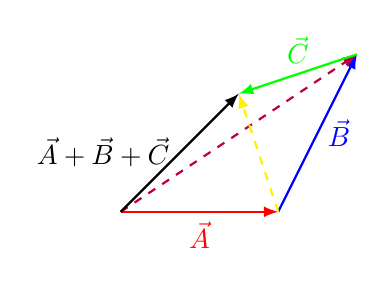
\begin{tikzpicture}[scale=1, transform shape]
            \draw[red,thick,-{latex}] (0,0) -- (2,0) node[midway, below] {$\vec{A}$};
            \draw[blue,thick,-{latex}] (2,0) -- (3,2) node[midway, right] {$\vec{B}$};
            \draw[dashed,purple,thick,-{latex}] (0,0) -- (3,2);
            \draw[green,thick,-{latex}] (3,2) -- (1.5,1.5) node[midway, above] {$\vec{C}$};
            \draw[dashed,yellow,thick,-{latex}] (2,0) -- (1.5,1.5);
            \draw[thick,-{latex}] (0,0) -- (1.5,1.5) node[midway, left] {$\vec{A}+\vec{B}+\vec{C}$};
        \end{tikzpicture}
    \end{center}
    \caption{Associative property of vector sum.}%
    \label{fig:vector-sum-associative}
\end{figure}

We define the zero vector due to the usefulness of zero in normal arithmetic.

\begin{definition}[Zero Vector]
    \[
        \vec{v}+\vec{0}=\vec{v}
    .\]
\end{definition}

\begin{note}
    \begin{align*}
         \vec{0}  & \neq 0. \\
        |\vec{0}| &   =  0.
    .\end{align*}
\end{note}

We also want $\vec{v}+(-\vec{v})=\vec{0}$ to be true, which means that $-\vec{v}$ has to has the opposite sense of $\vec{v}$ but the same magnitude and direction, following the definition of addition and zero vector.

\subsubsection{Scalar multiplication}%
\label{ssub:vector-scalar-multiplication}

\begin{definition}[Scalar multiplication]
    $c \vec{v}$ is a vector which has a $|c|$ times the magnitude of $\vec{v}$ in the same direction, and the same sense only if $c>0$, otherwise, the opposite sense.
\end{definition}

\begin{note}
    \begin{align*}
         d\vec{a}          &=  \vec{a}d. \\
        c(\vec{a}+\vec{b}) &= c\vec{a}+c\vec{b}. \\
        (c+d)\vec{a}       &= c\vec{a}+d\vec{a}. \\
        c( d\vec{a} )      &= d(c\vec{a}).
    .\end{align*}
\end{note}
\change{Explain this.}

\subsubsection{Inner product}%
\label{ssub:vector-inner-product}

It is formulated to represent linear relations like $W=\vec{F} \cdot  \vec{r}$, where only the components of the two vectors that are parallel to each other are relevant.

\begin{figure}[htpb]
\begin{center}
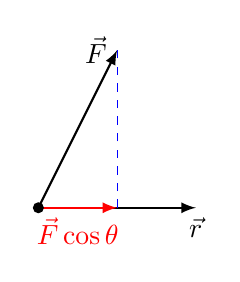
\begin{tikzpicture}[scale=1, transform shape]
    \draw[thick,-{latex}] (0,0) -- (2,0) node[below] {$\vec{r}$};
    \draw[thick,-{latex}] (0,0) -- (1,2) node[left] {$\vec{F}$};
    \draw[thick,-{latex},red] (0,0) -- (1,0) node[midway, below] {$\vec{F}\cos\theta$};
    \draw[dashed, blue] (1,0) -- (1,2);
    \fill (0,0) circle (2pt);
\end{tikzpicture}
\end{center}
\caption{Inner product applied on work.}%
\label{fig:work-inner-product}
\end{figure}

\begin{figure}[htpb]
    \begin{center}
        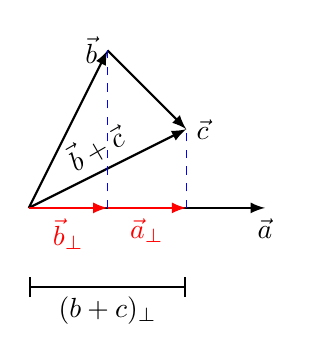
\begin{tikzpicture}[scale=1, transform shape]
            \draw[thick,-{latex}] (0,0) -- (3,0) node[below] {$\vec{a}$};
            \draw[thick,-{latex}] (0,0) -- (1,2) node[left] {$\vec{b}$};
            \draw[thick,-{latex}] (1,2) -- (2,1) node[right] {$\vec{c}$};
            \draw[thick,-{latex}] (0,0) -- (2,1) node[midway, above,rotate=30] {$\vec{b}+\vec{c}$};
            \draw[thick,-{latex},red] (0,0) -- (1,0) node[midway, below] {$\vec{b}_\perp$};
            \draw[thick,-{latex},red] (1,0) -- (2,0) node[midway, below] {$\vec{a}_\perp$};
            \draw[thick,|-|] (0,-1) -- (2,-1) node[midway, below] {$(b+c)_\perp$};
            \draw[dashed, blue] (1,0) -- (1,2);
            \draw[dashed, blue] (2,0) -- (2,1);
            % \fill (0,0) circle (2pt);
        \end{tikzpicture}
    \end{center}
    \caption{Distributive property of inner product.}%
    \label{fig:inner-product-distributive}
\end{figure}

\[
    \vec{a} \cdot ( \vec{b} + \vec{c} ) = \vec{a}\cdot\vec{b} + \vec{a}\cdot\vec{c}
.\]

\begin{definition}[Inner product]
    \[
        \vec{a} \cdot \vec{b} = |a| |b| \cos\theta
    .\]
\end{definition}

\begin{note}
    Inner product results in a scalar. Thus, it can \textbf{not} be \textit{commutative} ($\vec{a}\cdot \vec{b}\cdot \vec{c}$ is meaningless by definition). However, it \textbf{is} \textit{associative} ($\vec{a}\cdot \vec{b}=\vec{b}\cdot \vec{a}$).
\end{note}

\subsubsection{Outer product}%
\label{ssub:vector-outer-product}

In contrast to inner product, outer product is formulated to represent rotational relations like $\vec{\tau} = \vec{F} \wedge \vec{r}$, where only the components of the two vectors that are perpendicular to each other are relevant.

However, it creates a new mathematical object, the bivector, which is oriented plane segment like how vectors are oriented line segments. They are related to pseudovectors in physics (e.g. angular velocity).

\[
    \vec{a}\wedge \vec{b}=\bivec{B}
.\]

\begin{figure}[htpb]
\begin{center}
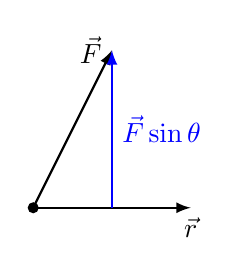
\begin{tikzpicture}[scale=1, transform shape]
    \fill (0,0) circle (2pt);
    \draw[thick,-{latex}] (0,0) -- (2,0) node[below] {$\vec{r}$};
    \draw[thick,-{latex}] (0,0) -- (1,2) node[left] {$\vec{F}$};
    \draw[thick,-{latex},blue] (1,0) -- (1,2) node[midway, right] {$\vec{F}\sin\theta$};
\end{tikzpicture}
\end{center}
\caption{Outer product applied on torque.}%
\label{fig:torque-outer-product}
\end{figure}

\begin{definition}[Outer product]
    \[
        |\vec{a} \wedge \vec{b}| = |a| |b| \sin\theta
    .\]
\end{definition}

\begin{figure}[H]
    \begin{center}
        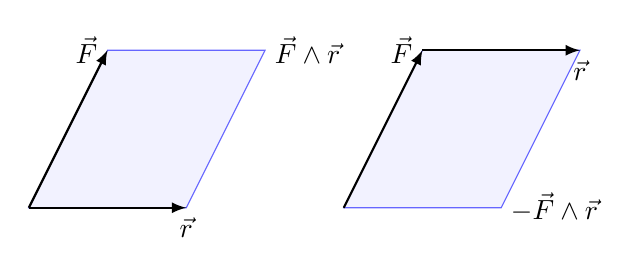
\begin{tikzpicture}[scale=1, transform shape]
            \filldraw[color=blue!60, fill=blue!5] (0,0) -- (1,2) -- (3,2) node[black, right] {$\vec{F}\wedge\vec{r}$} -- (2,0) -- cycle;
            \draw[thick,-{latex}] (0,0) -- (2,0) node[below] {$\vec{r}$};
            \draw[thick,-{latex}] (0,0) -- (1,2) node[left] {$\vec{F}$};
            \node [scale=3] at (1.5,1) {$\circlearrowright$};

            \filldraw[color=blue!60, fill=blue!5] (4,0) -- (5,2) -- (7,2) -- (6,0) node[black, right] {$-\vec{F}\wedge\vec{r}$} -- cycle;
            \draw[thick,-{latex}] (5,2) -- (7,2) node[below] {$\vec{r}$};
            \draw[thick,-{latex}] (4,0) -- (5,2) node[left] {$\vec{F}$};
            \node [scale=3] at (5.5,1) {$\circlearrowleft$};
        \end{tikzpicture}
    \end{center}
    \caption{The bivector result of outer product.}%
    \label{fig:bivector-result}
\end{figure}

The difference between clockwise and counterclockwise is represented through the anticommutative property ($\vec{a}\wedge\vec{b}=-\vec{b}\wedge \vec{a}$).

\begin{figure}[htpb]
    \centering
    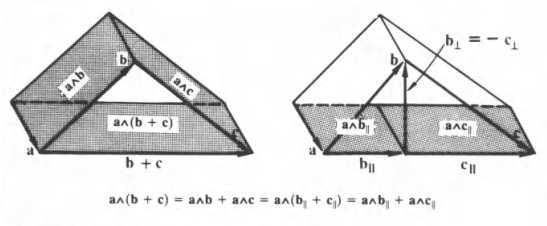
\includegraphics[width=0.8\textwidth]{figures/bivectors-dist.PNG}
    \caption{Distributive property of outer product}
    \label{fig:outer-product-distributive}
\end{figure}

\begin{align*}
    \vec{b} + \vec{c} &= (\vec{b}_\parallel+\vec{b}_\perp) + (\vec{c}_\parallel+\vec{c}_\perp) \\
    &= (\vec{b}_\parallel+\vec{b}_\perp) + (\vec{c}_\parallel-\vec{b}_\perp) \\
    &= \vec{b}_\parallel + \vec{c}_\parallel
.\end{align*}
\begin{align*}
    \vec{a} \wedge ( \vec{b} + \vec{c} ) &= \vec{a} \wedge (\vec{b}_\parallel + \vec{c}_\parallel) \\
                                         &= \vec{a} \wedge \vec{b}_\parallel + \vec{a} \wedge \vec{c}_\parallel \\
                                         &= \vec{a} \wedge \vec{b} + \vec{a} \wedge \vec{c}
.\end{align*}

The next step after bivectors is trivectors. Just like vectors and bivectors but for three dimensions, they are oriented volume. In addition, they are closely related to pseudoscalers in physics (e.g. magnetic flux).

\[
    ( \vec{a} \wedge \vec{b} ) \wedge  \vec{c} = \trivec{T}
.\]

However, we do not define tetravectors (4-vectors) because they are not helpful in the \textit{current} dimensional space.

\begin{align*}
    ( ( \vec{a} \wedge \vec{b} ) \wedge  \vec{c} ) \wedge \vec{d} &= 0 \\
    \vec{a} \wedge \vec{b} \wedge  \vec{c} \wedge \vec{d} &= 0 \\
    \trivec{T} \wedge \vec{d} &= 0
.\end{align*}

\begin{figure}[htpb]
    \centering
    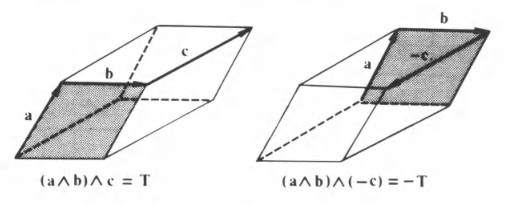
\includegraphics[width=0.8\textwidth]{figures/trivectors.PNG}
    \caption{The trivector result of outer product.}
    \label{fig:trivetors}
\end{figure}

\begin{note}
    Outer product is associative: $( \vec{a}\wedge \vec{b} )\wedge \vec{c}=\vec{a}\wedge (\vec{b}\wedge \vec{c})$.
\end{note}
\change{Explain this.}

\subsubsection{Geometric product}%
\label{ssub:geometric-product}

While the inner product captures the parallelism between vectors and the outer product captures the perpendicularity between vectors, none captures both. Therefore, the formulation of geometric product is needed.

\begin{definition}
    \[
    \vec{a}\vec{b}=\vec{a}\cdot\vec{b} + \vec{a}\wedge\vec{b}
    .\]
\end{definition}

It is simply defined as their sum, although they are different mathematical objects, similar to how we define complex numbers ($a+bi$). Following this definition we conclude the geometric product properties.

\begin{align*}
    \vec{a}\vec{b} &\neq \vec{b}\vec{a} \\
                   &= \vec{a}\cdot \vec{b}-\vec{b}\wedge \vec{a}
.\end{align*}

\begin{align*}
    \vec{a}(\vec{b}+\vec{c}) &= a\cdot(b+c) + a\wedge(b+c) \\
                             &= ( a\cdot b + a\wedge b ) + ( a\cdot c + a\wedge c ) \\
                             &= \vec{a}\vec{b} + \vec{a}\vec{c}
.\end{align*}

\[
    c \vec{a}\vec{b}=(c \vec{a})\vec{b} = a(c \vec{b})
.\]

\begin{align*}
    \vec{a}\vec{b}+\vec{b}\vec{a} &= ( a \cdot b + \vec{a}\wedge \vec{b} ) + ( b \cdot a - \vec{a}\wedge \vec{b} ) \\
                                  &= 2 a \cdot b \\
    \therefore \vec{a} \cdot \vec{b} &= \frac{1}{2}(\vec{a}\vec{b}+\vec{b}\vec{a})
.\end{align*}

\begin{align*}
    \vec{a}\vec{b}-\vec{b}\vec{a} &= ( a \cdot b + \vec{a}\wedge \vec{b} ) + ( - b \cdot a + \vec{a}\wedge \vec{b} ) \\
                                  &= 2 \vec{a} \wedge \vec{b} \\
    \therefore \vec{a} \wedge \vec{b} &= \frac{1}{2}(\vec{a}\vec{b}-\vec{b}\vec{a})
.\end{align*}

\subsubsection{Geometric division}%
\label{ssub:geometric-division}

Now we can define geometric division as $\trivec{A_k}^{-1}\trivec{A_k}=1$, where $A_k$ is a multivector, and follow to conclude a formula.

\begin{align*}
    \trivec{A_k}^{-1}\trivec{A_k}&=1 \\
    \trivec{A_k}^{-1}\trivec{A_k}\trivec{A_k}&=\trivec{A_k} \\
    \trivec{A_k}^{-1}\trivec{A_k}^2&=\trivec{A_k} \\
    \trivec{A_k}^{-1}|\trivec{A_k}|^2&=\trivec{A_k} \\
    \trivec{A_k}^{-1}&=\frac{\trivec{A_k}}{|\trivec{A_k}|^2} \\
.\end{align*}

\begin{note}
    \begin{align*}
        A_kA_k&=A_k^2 \\
              &=A_k \cdot A_k + A_k \wedge  A_k \\
              &=|A_k| |A_k| \cos 0 + |A_k| |A_k| \sin 0 \\
              &=|A_k| |A_k| + 0 \\
              &=|A_k|^2
    .\end{align*}
\end{note}

\newpage
